
\section{NOTES--Allen}

% \subsection{graphics}
% 
% 
% \begin{figure}[h]
% 	\begin{center}
% 	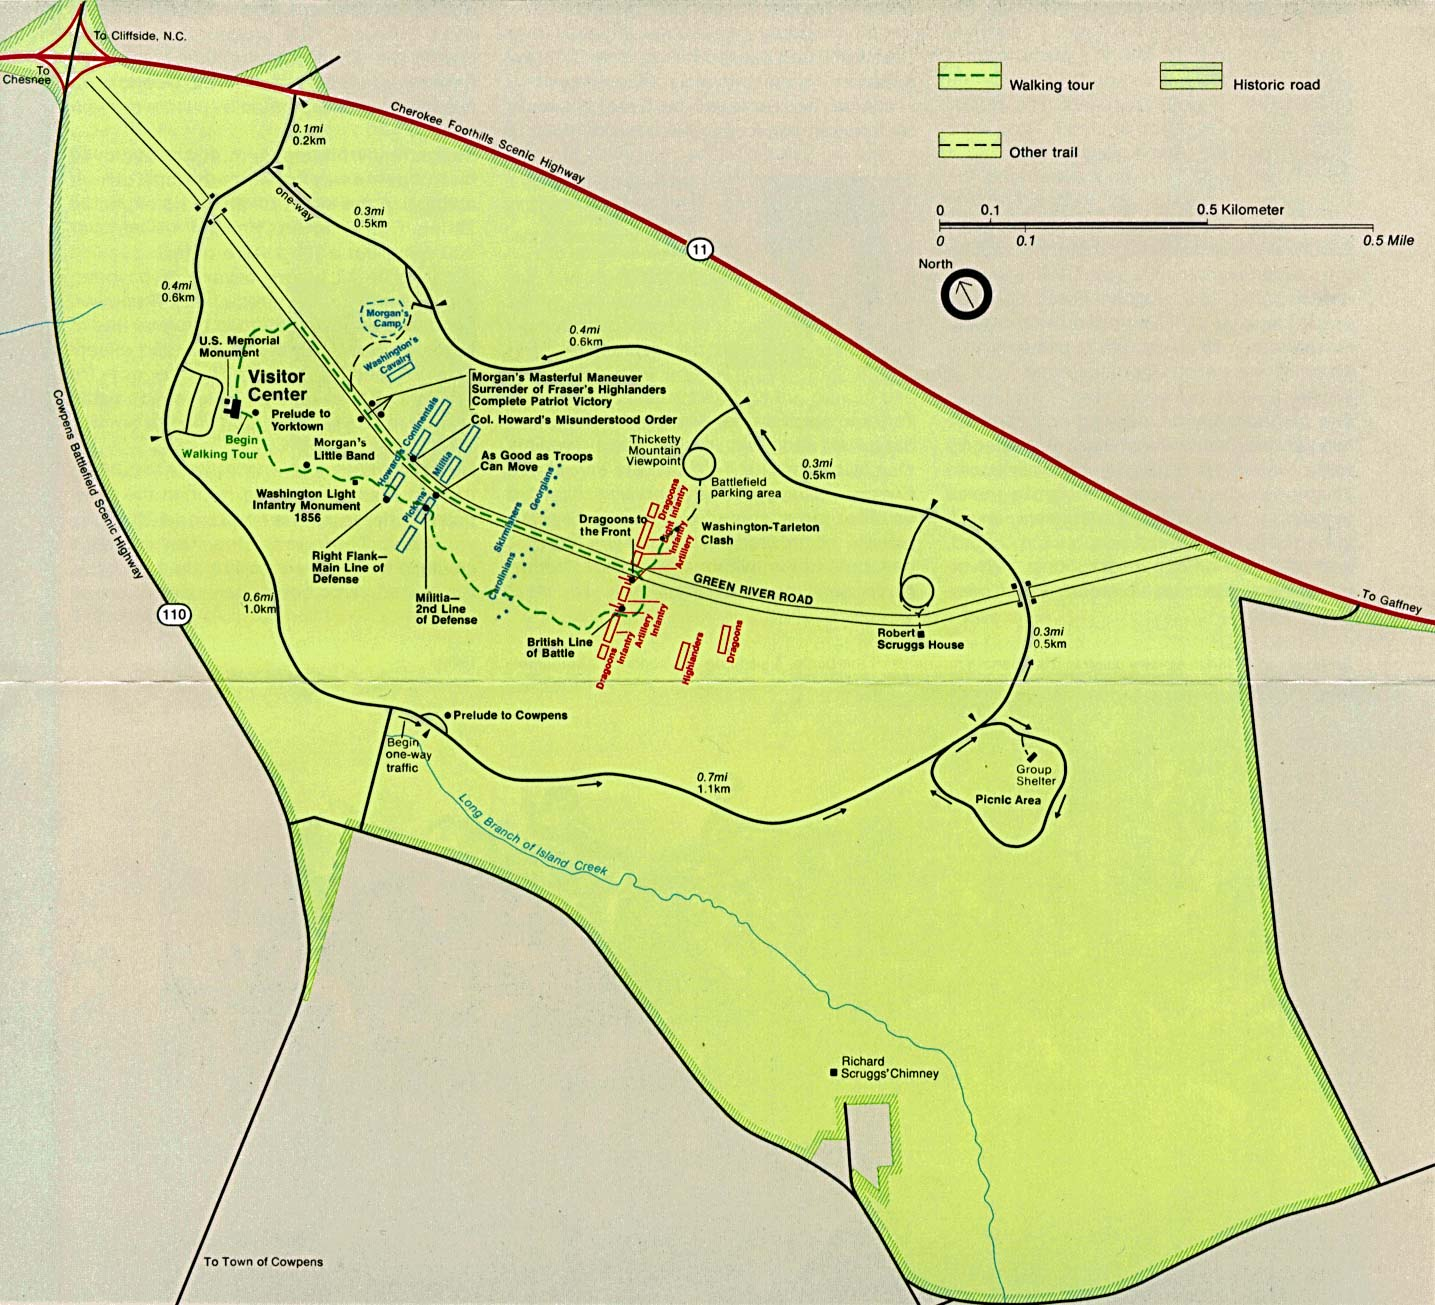
\includegraphics[width=6in]{gfx/cowp_95}
% 	\end{center}
% 	\caption{This is a caption}
% 	\label{cowpbatt95}
% \end{figure}
% 
% 
% 
% \begin{figure}[h]
% 	\begin{center}
% 	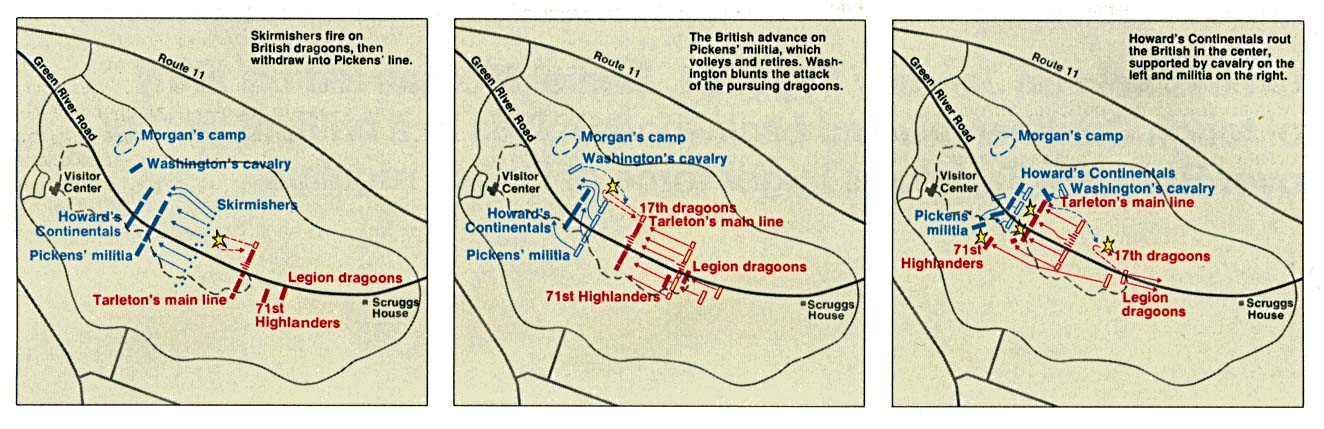
\includegraphics[width=6in]{gfx/cowp_batt95}
% 	\end{center}
% 	\caption{This is a caption}
% 	\label{cowp95}
% \end{figure}
% 
% 
% \begin{figure}[h]
% 	\begin{center}
% 	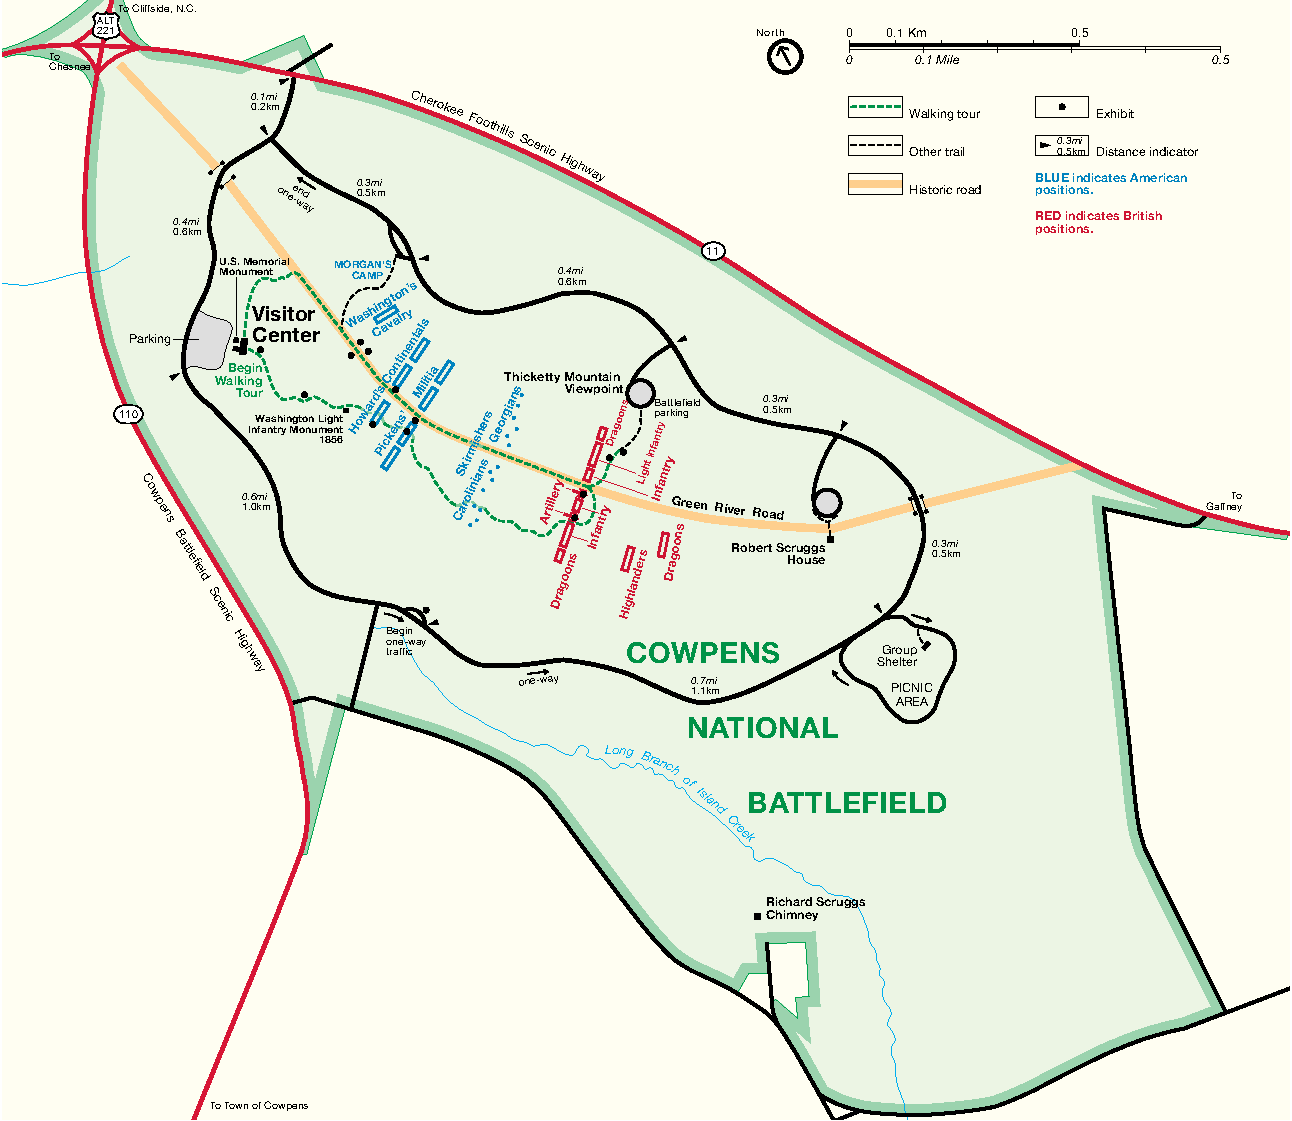
\includegraphics[width=6in]{gfx/cowpens_park97}
% 	\end{center}
% 	\caption{Cowpens National Battlefield.}
% 	\label{cowppark97}
% \end{figure}
% 
% 
% \begin{figure}[h]
% 	\begin{center}
% 	  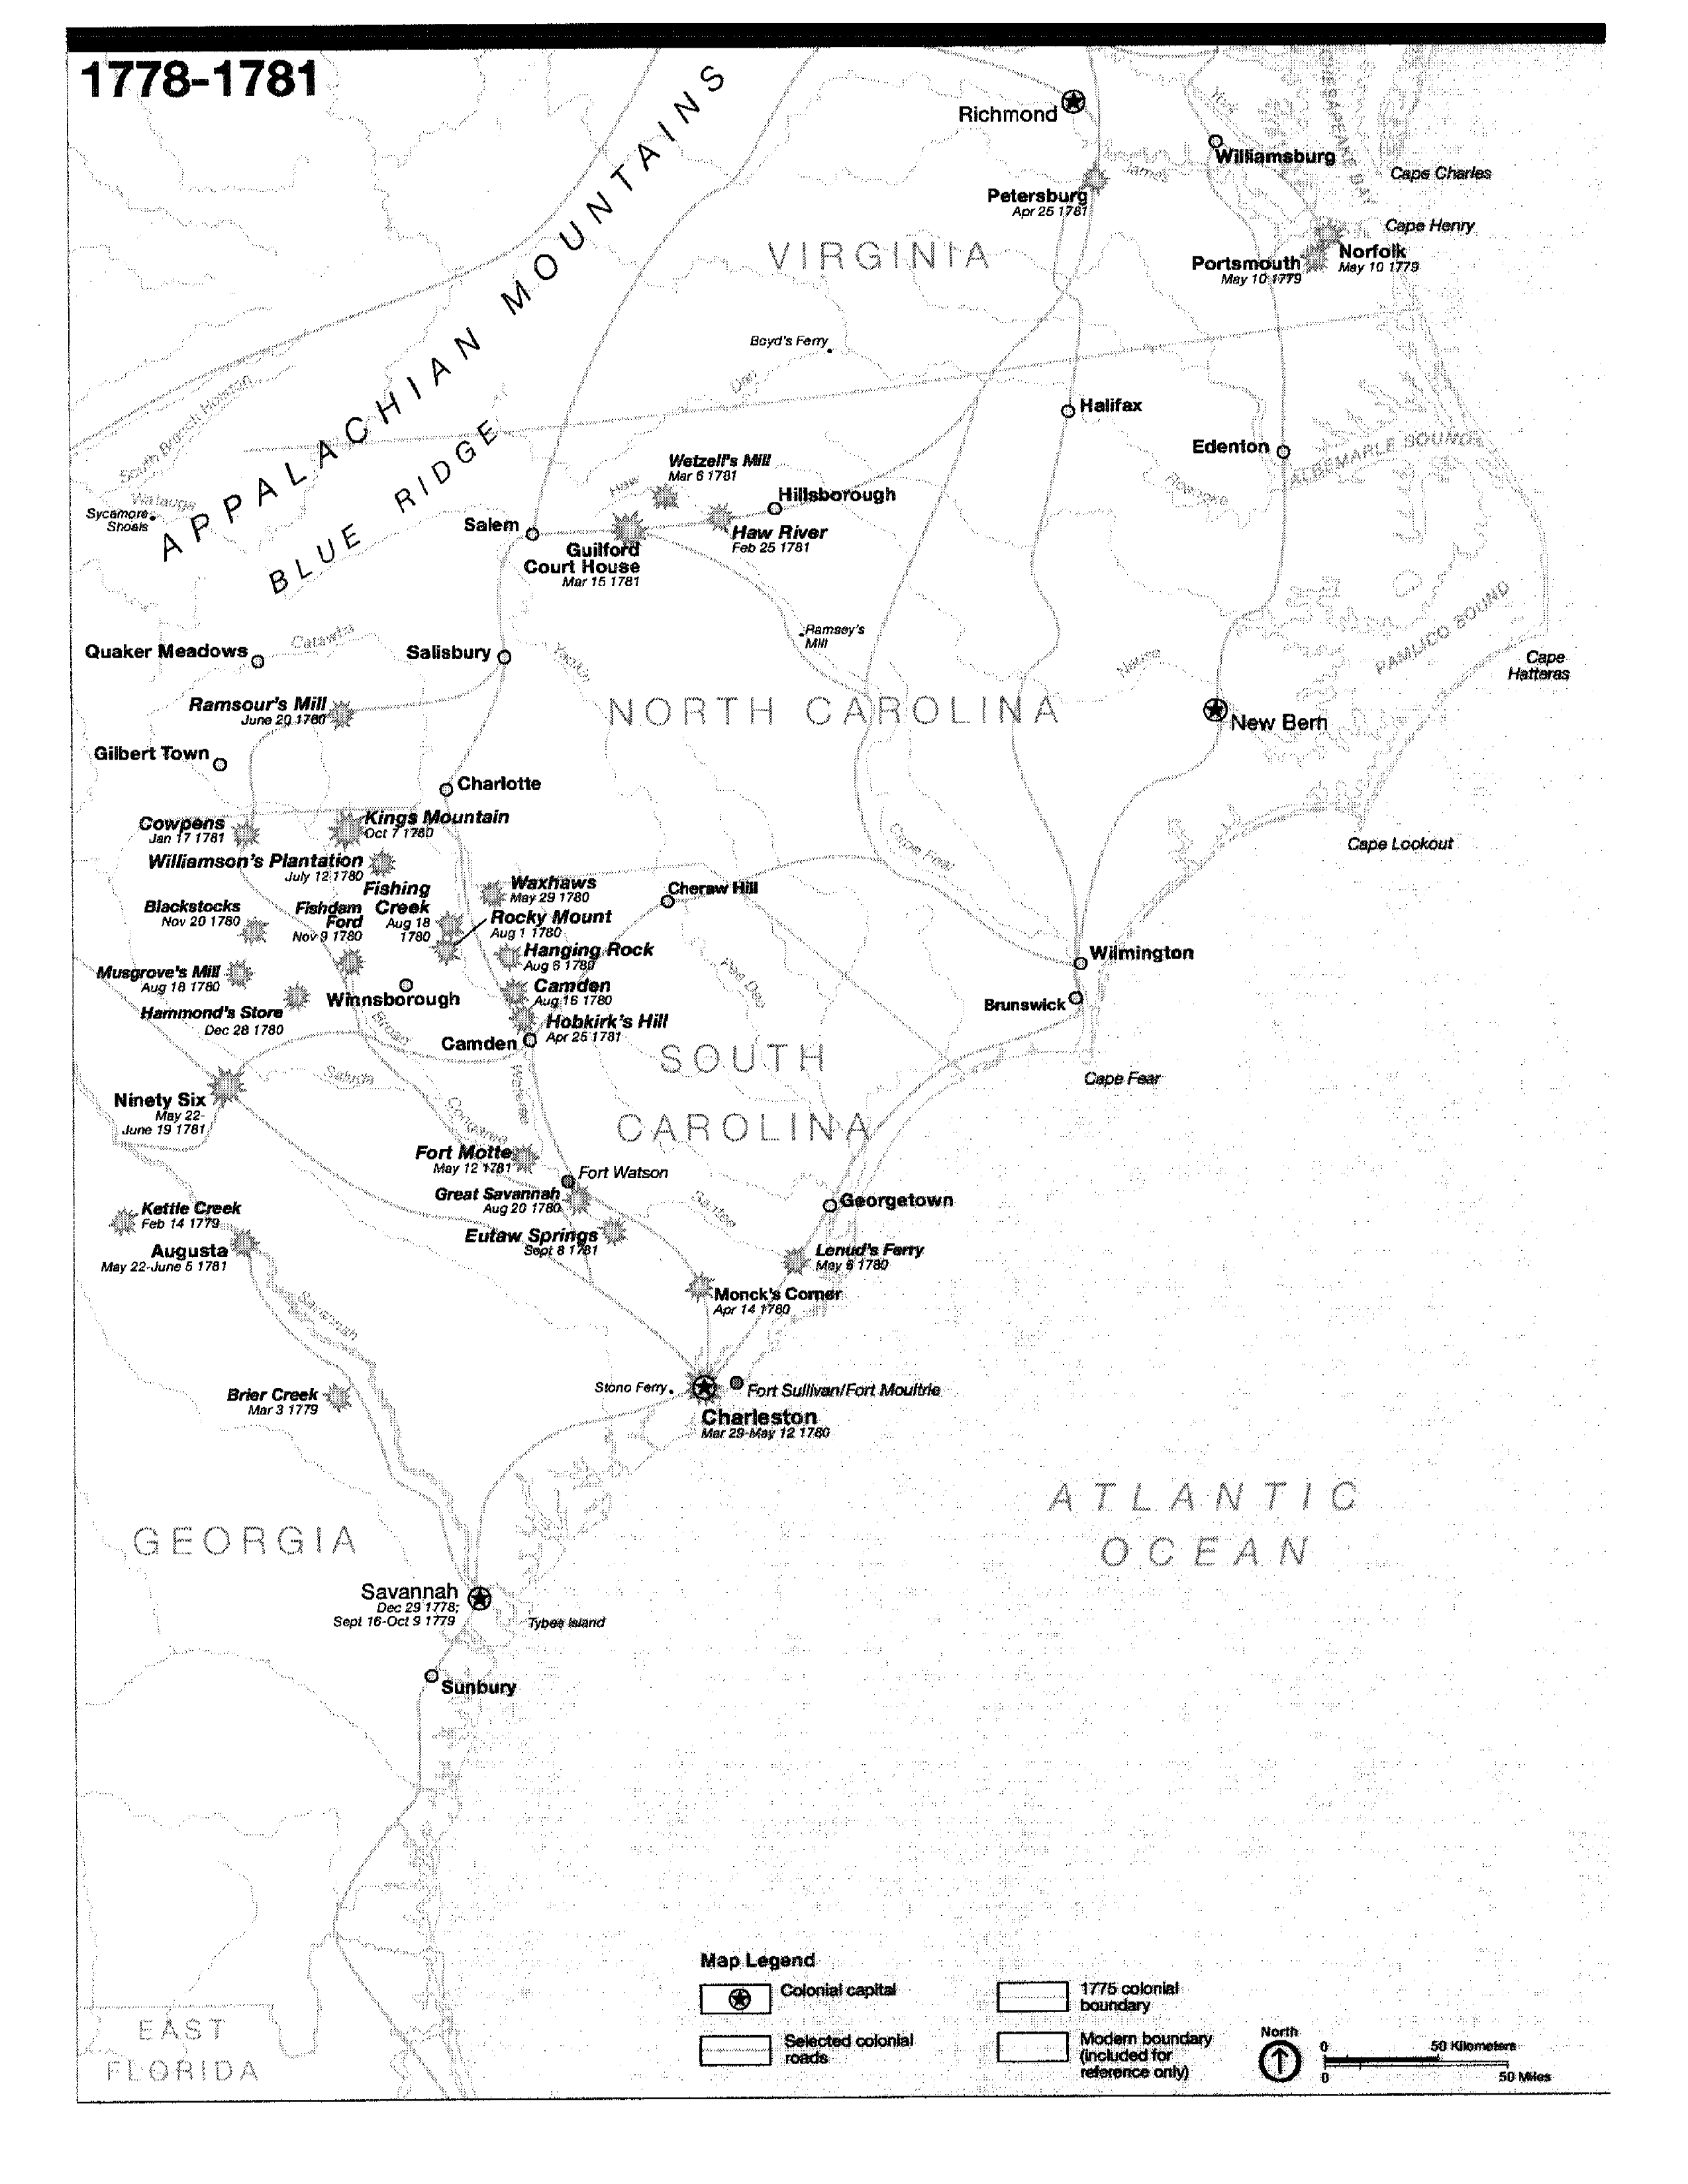
\includegraphics[width=6in]{gfx/rauch_battle_2007_01_p18}
% 	\end{center}
% 	\caption{\cite[18]{rauch_battle_2007}}
% 	\label{cowppark97}
% \end{figure}
% 
% \begin{figure}[h]
% 	\begin{center}
% 	  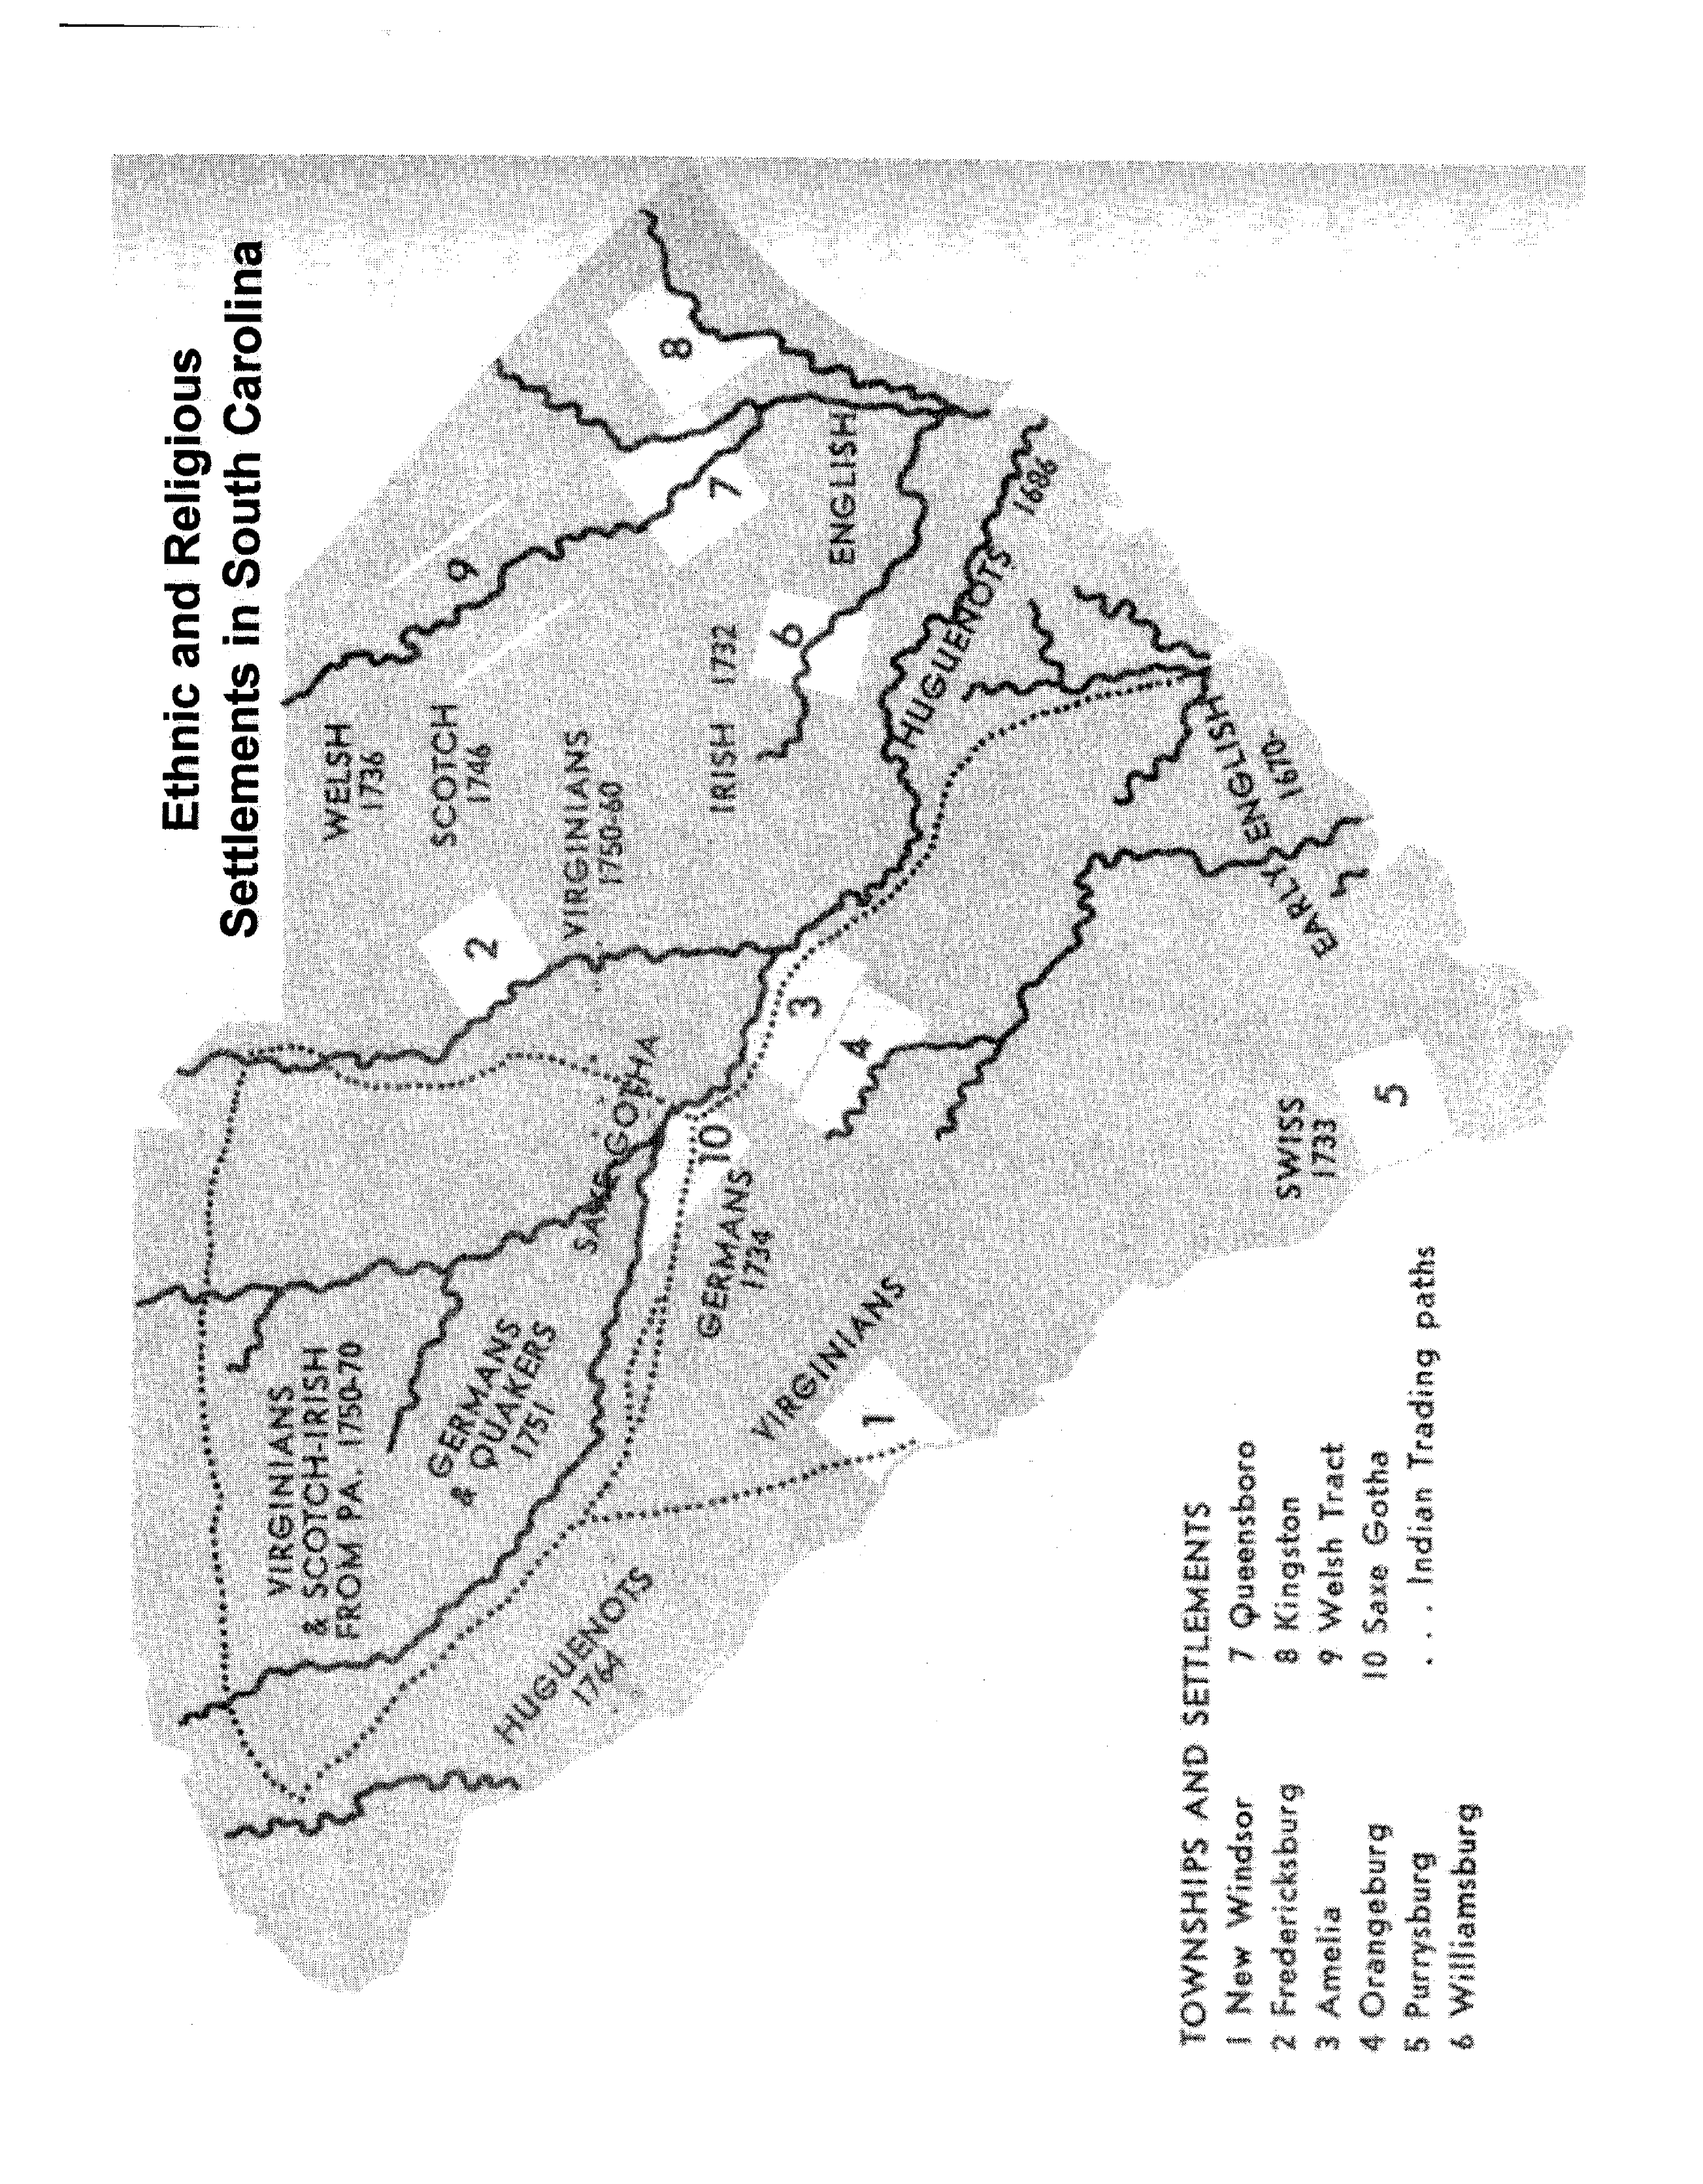
\includegraphics[angle=-90,width=4in]{gfx/rauch_battle_2007_02_p19}
% 	\end{center}
% 	\caption{Cowpens National Battlefield.}
% 	\label{cowppark97}
% \end{figure}
% 
% \begin{figure}[h]
% 	\begin{center}
% 	  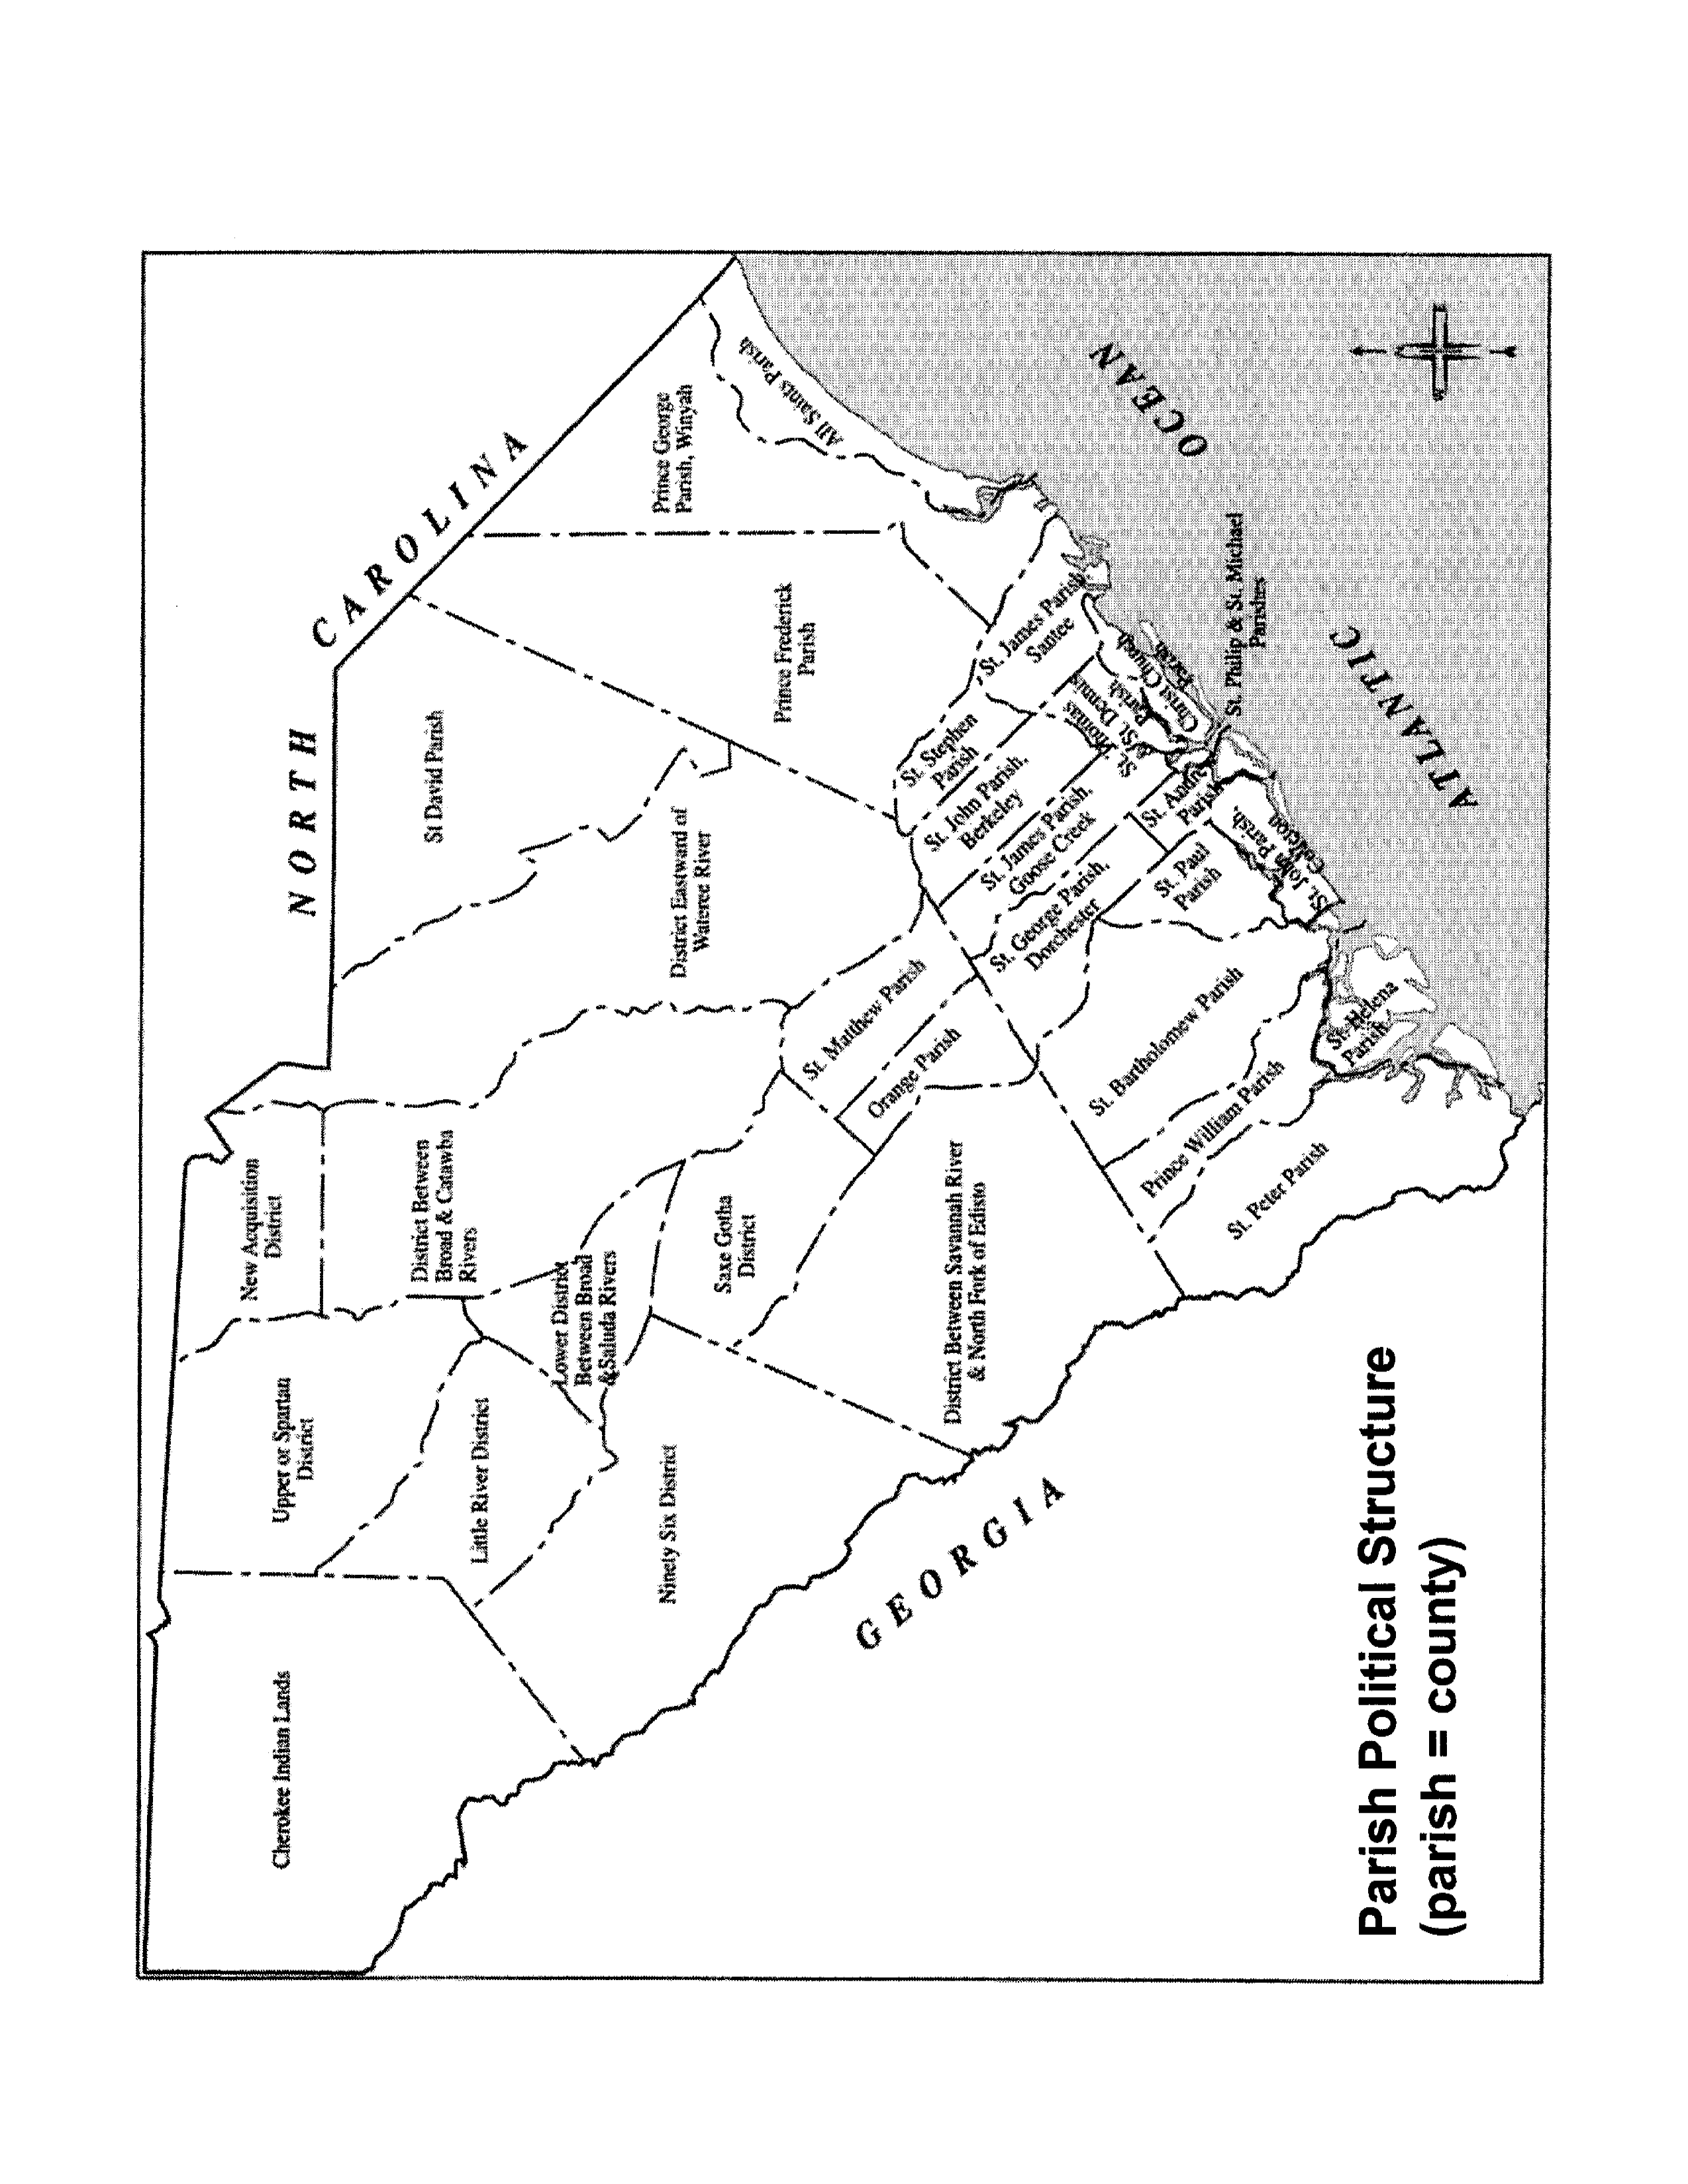
\includegraphics[angle=-90,width=6in]{gfx/rauch_battle_2007_03_p20}
% 	\end{center}
% 	\caption{Cowpens National Battlefield.}
% 	\label{cowppark97}
% \end{figure}
% 
% \begin{figure}[h]
% 	\begin{center}
% 	  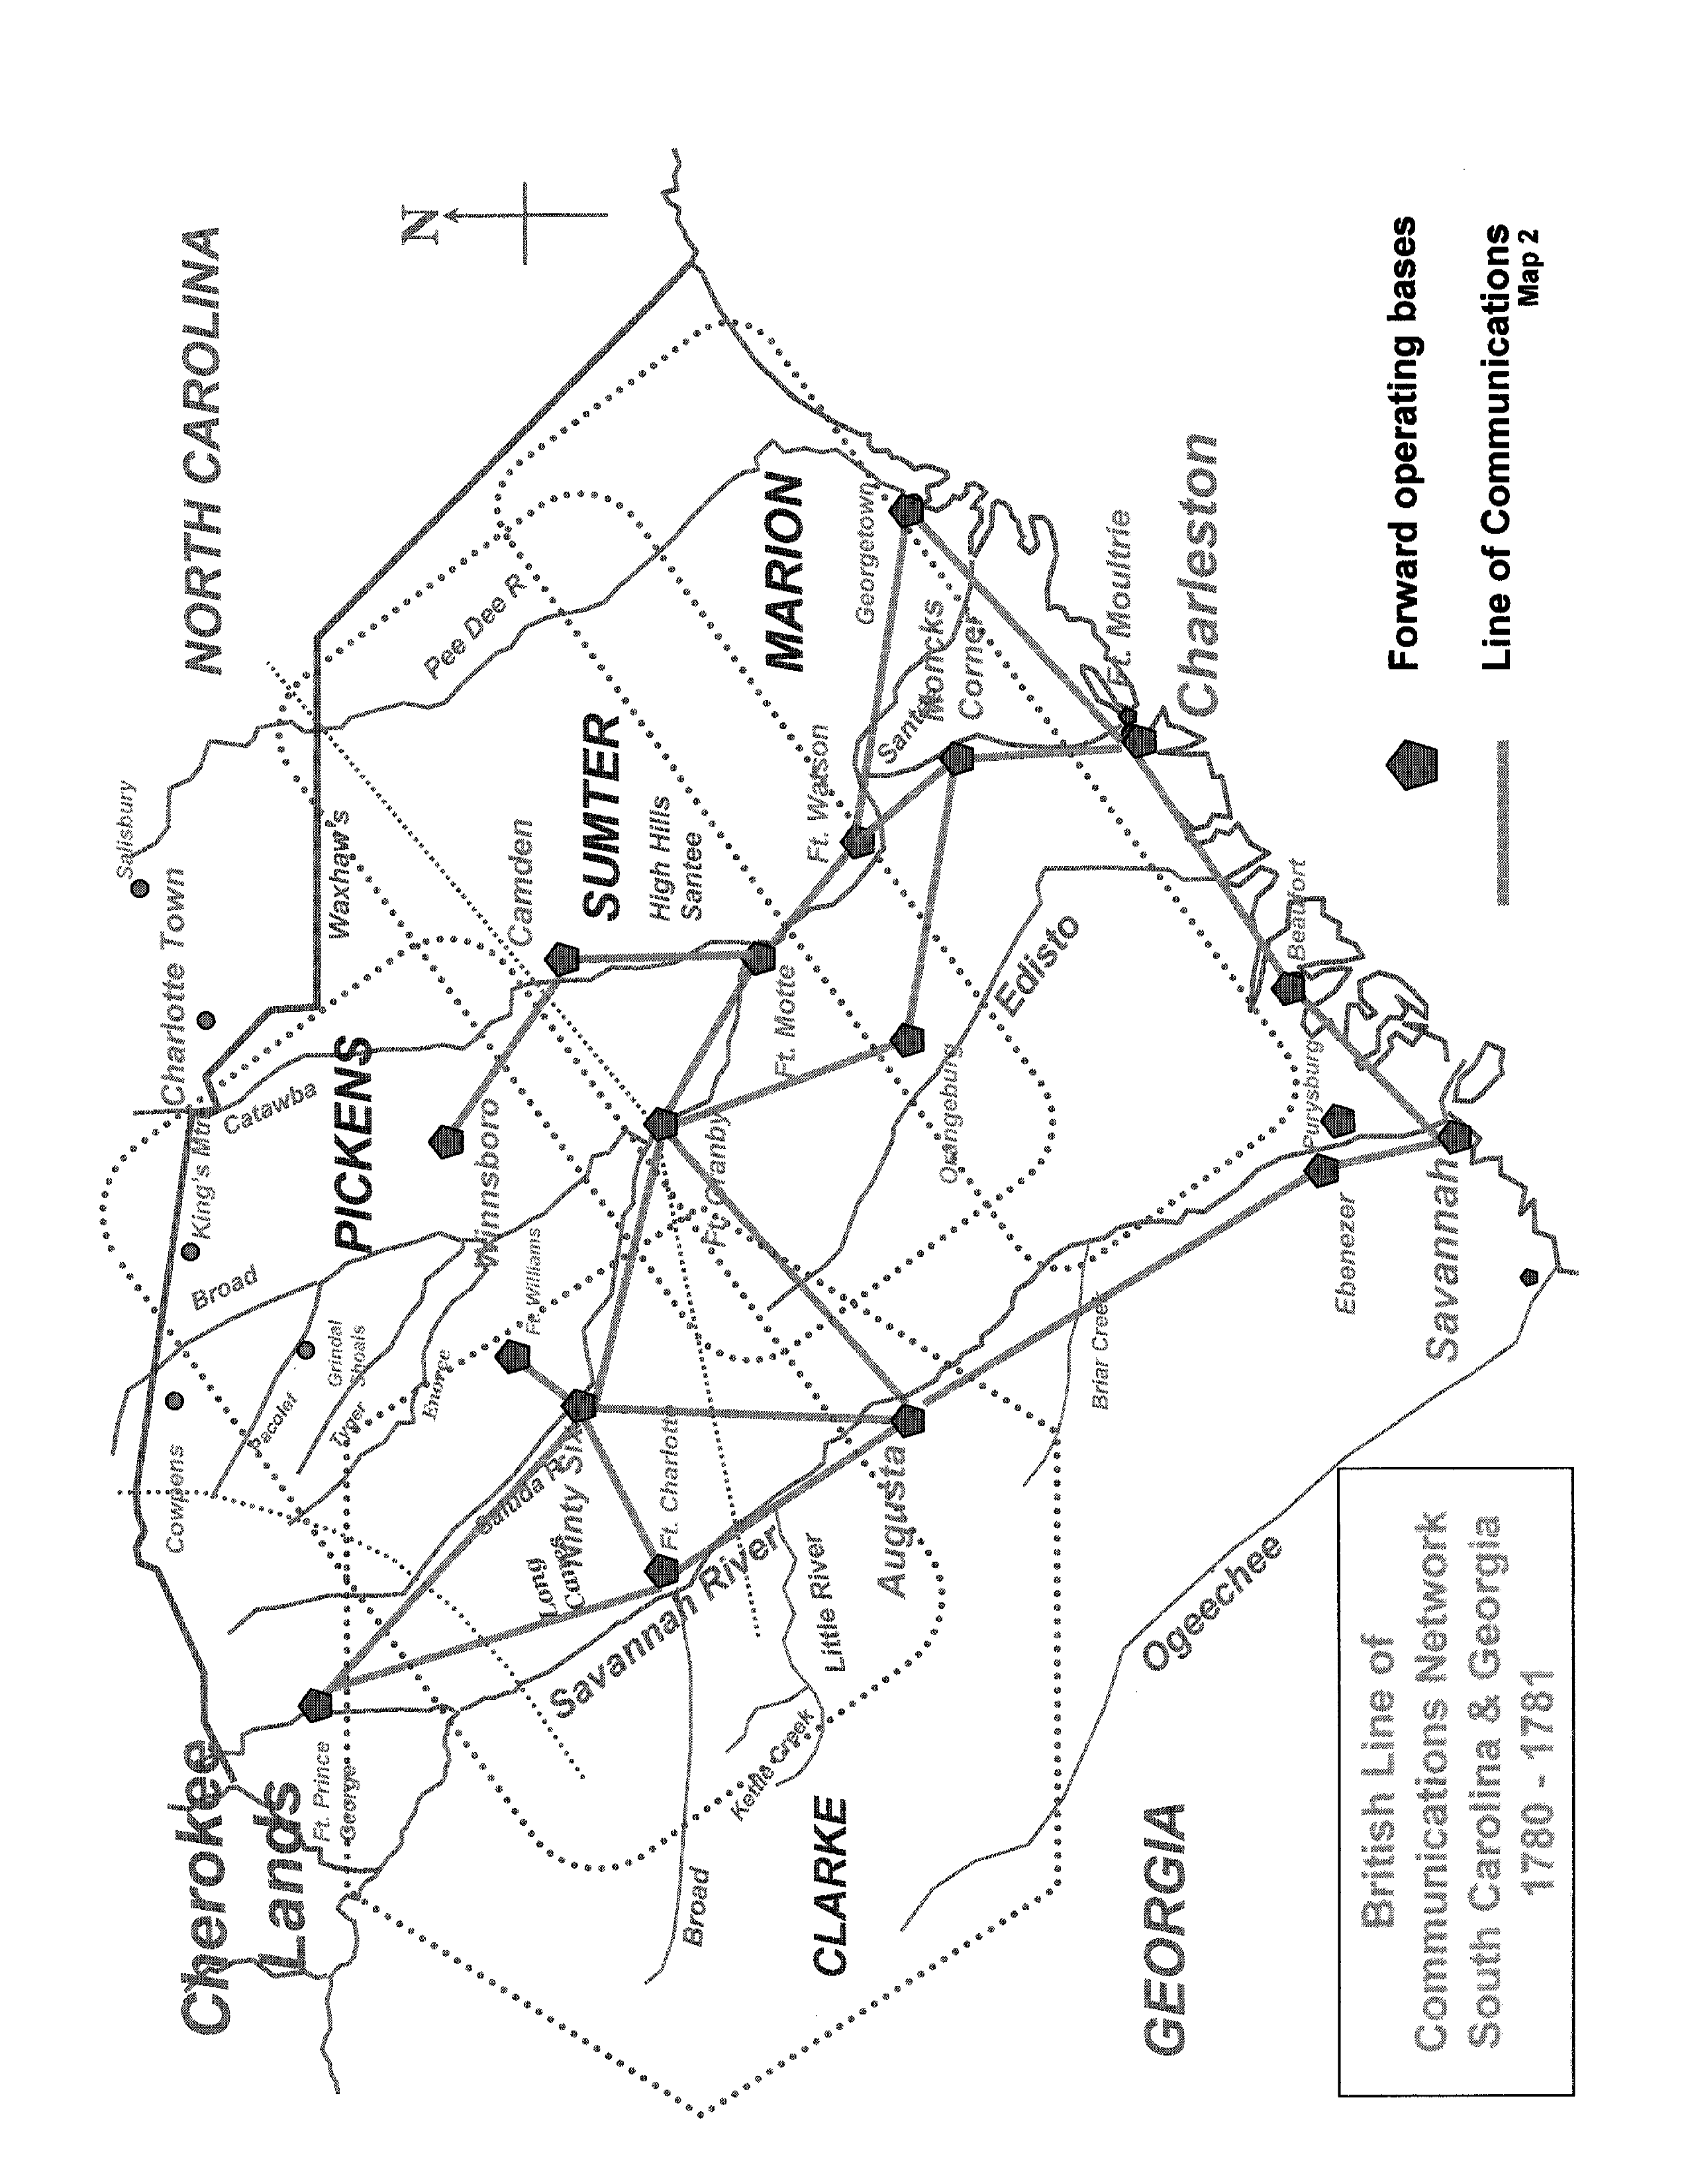
\includegraphics[angle=-90,width=6in]{gfx/rauch_battle_2007_04_p21}
% 	\end{center}
% 	\caption{Cowpens National Battlefield.}
% 	\label{cowppark97}
% \end{figure}
% 
% \begin{figure}[h]
% 	\begin{center}
% 	  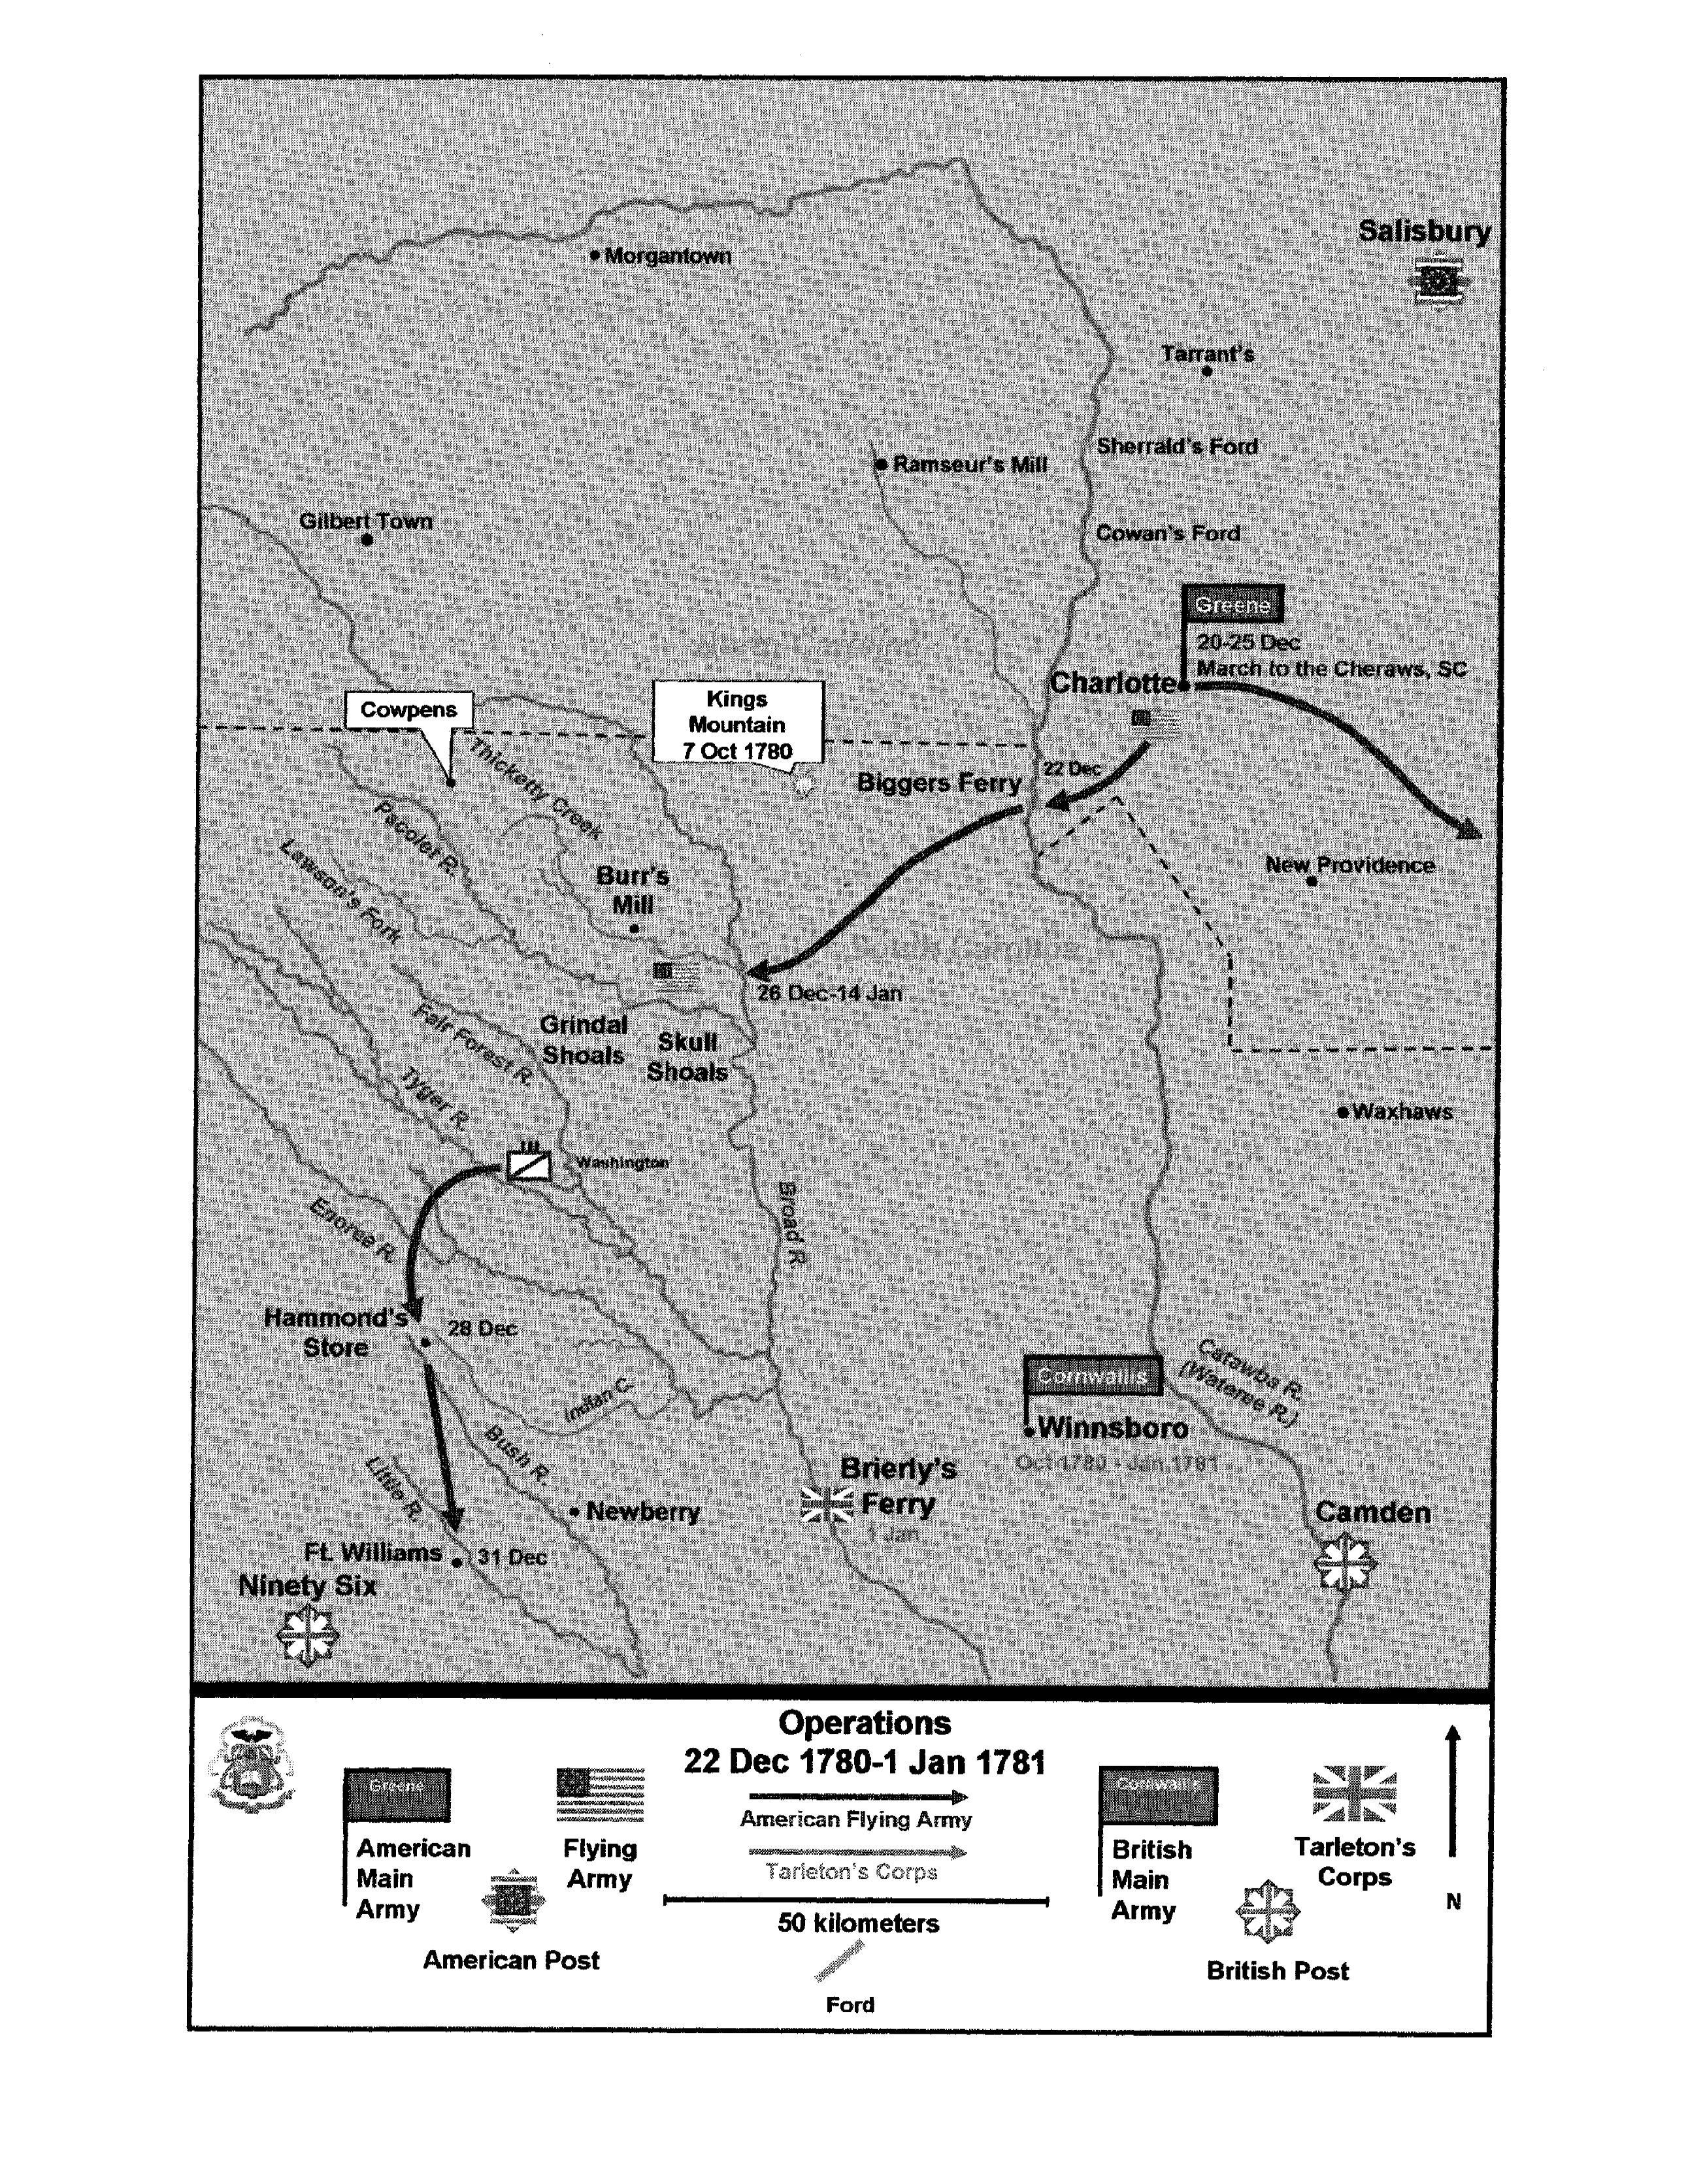
\includegraphics[width=6in]{gfx/rauch_battle_2007_05_p22}
% 	\end{center}
% 	\caption{Cowpens National Battlefield.}
% 	\label{cowppark97}
% \end{figure}
% 


\subsection{notes: British Army}

``At the outbreak o fthe Revolution, the total land forces of Great Britain
exclusive of militia numbered on paper 48,647 men, of which 39,294 were
infantry; 6,869 cavalry; and 2,484 artillery. These troops were unequally
divided between two separate military establishments--the English establishment
and the Irisih establishment. \ldots

Such were the numbers of the British army in 1775 and such they had
approximately been ever since the close of the Seven Years' War.''\footcite[1]{curtis_org_1972}

``An examination of the location of the British army in 1775 reveals the fact
that while small detachments of it were to be found in many distant quarters of
the globe, the bulk of it was distributed unequally among three different
countries. There were roughly speaking 15,000 men in England, 12,000 in
Ireland, and 8,000 in America. The remaining 10,000 were distributed among the
West Indes, Africa, Minorca, Gibraltar, and
Scotland.''\footcite[2]{curtis_org_1972}

\red{See \footcite[4]{curtis_org_1972} for discussion of \emph{Light Infantry} and
\emph{Grenadiers} in the British Army}

``The uniform of the private soldier was ill adapted for comfort and speedy
movement. \ldots Over his left shoulder the foot soldier wore a broad belt
supporting a cartouch box, while another belt around this waist supported a
bayonet and short sword. On service the infantryman also carried a knapsack
containing extra clothing and brush and blackball, a blanket, a haversack with
provisions, a canteen, and a fifth share of the general equipage belonging to
his tent. These articles (estimating the provision to be for four days) added
to his accoutrements, arms, and sixty rounds of ammunition made, according to
Burgoyne, a bulk totally incompatible with combat and a weight of about sixty
pounds.''\footcite[14-15]{curtis_org_1972}

``The British regular fought the embattled farmers of America with the `Brown
Bess.' This was a smoothbore flintlock musket with a priming pan, three feed
eight inches long in the barrel, and weighing fourteen pounds. It had an
effective range of three hundred yards, but its accuracy was unreliable at a
distance greater than one hundred. A soldier who could hit his enemy at that
interval must have been a first-class marksman and have possessed a Brown Bess
of exceptionally good quality. At a distance of over one hundred yeards, the
firing line during an engagement relied not so much upon the shooting of each
individual as upon the general effect of the volleys it
delivered\ldots''\footcite[16]{curtis_org_1972}

Twelve separate motions were required to fire the Brown Bess, which a ``clever
marksman'' could fire five times a minute, but the average soldier managed two
to three rounds per minute.\footcite[17]{curtis_org_1972} ``With bayonets fixed,
only one rounds could be fired to much purpose; since the bayonet made it
difficult to ram down the charge.''\footcite[17]{curtis_org_1972}

\red{infantry highly dependant on weather: rain/wind can prevent
firing\footcite[19]{curtis_org_1972}}

``\ldots~marksmanship in most regiments was poor. Scant mention is made of target
practice, and the inference is that there was little of it. It has been climed
that the soldiers did not aim at anything in particular. This probably accounts
for the saying that it took a man's weight in bullets to kill him. An American
who was taken prisoner by the 42d Highlanders during the assault on Fort
Washington in 1776 relates: `Not less than ten guns were discharged with their
muzzles toward us, within forty or fifty yards, and some were let off within
twenty. \ldots I observed that they took no aim, and the moment of presenting
and firing was the same.' These conditions gave rise to the sharpshooter, a man
who not merely aimed this musket, but aimed it at something or somebody. During
the capaign of 1777, Burgoyne formed a body of shapshooters by selecting a group
of sober, active, robust men from each regiment. Officers trained in the school
of European warfare, however, were prone to place more eliance upon the bayonet
than upon the bullet. Burgoyne in particular urged his men to use the bayonet:
`Men of half [your] bodily strength and even Cowards may be [your] match in
firing; but the onset of Bayonets in the hands of the Valiant is irresistible.
\ldots It will be our glory and preservation to storm where possible.'
''\footcite[20-21]{curtis_org_1972}

American flints were also superior, both yeilding a more reliable spark, and
requiring sharpening after ever 60 rounds, compared to British flints after
six.\footcite[21]{curtis_org_1972}

\red{dicussion of the purchase system for commissions.\footcite[24-29]{curtis_org_1972}}

``By 1781 a force of 110,000 man had been enrolled, of which about 56,000 were
located in America and the West Indes.''\footcite[51]{curtis_org_1972} Recruiting
was difficult, as the British army made attempts to recruit out of it's own
militias, hiring of Hessians, and recruting of Germans, Roman Catholics
(previously excluded until 1775),and attempts in 1775 to procure 20,000
mercenaries from Russia.\footcite[52]{curtis_org_1972} 


\subsection{notes}

\url{http://www.cgsc.edu/carl/download/csipubs/WarTermination2010.pdf}

\fullcite{gruber_2010}

On New Year's Day of 1781, the War for American Independence was in its sixth
year with no end in sight. The war had begun in 1775 when the British
government used force in Massachusetts to put down a rebellion that had been
building in its North American colonies for more than a decade. Fighting soon
spread from Massachusetts to other British colonies on the Atlantic seaboard
from New Hampshire to South Carolina. By the summer of 1776, the colonists had
raised a Continental army, declared their independence, created republican
state governments, and come together in a loose confederation of states to wage
war and conduct foreign affairs. When American forces captured a British army
at Saratoga, New York, in fall of 1777, the new United States secured both
treaties and an alliance with France, turning their war of independence into a
world war. The British had to fight not just their former colonists but also
France, Spain, and the Netherlands in a war that stretched from North America
to the West Indies, the English Channel, the Mediterranean Sea, and the coasts
of Africa and India. In North America, the British managed to carry on the war
with smaller regular forces and had some success maintaining a base at New York
City, capturing Savannah and Charleston, and by 1780 establishing posts from
the interior of Georgia and South Carolina to the Chesapeake. Even after
promising not to tax the colonists or to interfere in their internal affairs,
the British had not been able to restore royal government anywhere beyond the
reach of their armies nor had the Americans been able to exploit the
opportunities that had come with a wider war such as to raise the forces needed
to cooperate effectively with French squadrons that reached North America each
year or to take advantage of the reduction and redeployment of the British
fleet and army in the United States. Indeed, at New Year's Day in 1781, the war
seemed far from over. No one could have predicted confidently that 1781 would
have the final campaign of the War for American Independence.

The war had dragged on indecisively in America because each side had great
difficulty in using force to achieve its war aims. The British had never been
able to find a combination of force and persuasion to restore royal government
beyond a few ports and outposts. The new United States had had nearly as much
difficulty as the British in using force. Since 1776, Americans had fought for
independence, a national domain, and republican government.  Having rebelled
against a remote and oppressive imperial administration, Americans were also
determined to win their independence without creating a central government or a
standing army that could coerce the states or deprive the people of their
liberties.  They hoped first to defeat the British with an army of short-term
volunteers supported by militiamen and supplied by the states, but the campaign
of 1776 at New York made it clear that such forces could not wage war
successfully against the British regular army. Congress agreed to strengthen
the Continental Army by enlisting men for at least three years and by adopting
a code of military discipline that would help turn raw recruits into effective
soldiers, measures that significantly improved the army by the spring of 1778. Even so,
without the power to tax, Congress had to depend on loans from European nations and
contributions from the American states to pay, feed, clothe, house, and arm its forces and
those loans and contributions were rarely adequate. Continental soldiers who were hungry
and unpaid went home or mutinied with increasing frequency after 1779, and American
commanders were forced to limit their operations and to rely more than they wished on
poorly trained and wasteful militia. They were never able to cooperate adequately with the
French squadrons that came to North America each year from 1778 to 1780.

Although Congress and the Continental Army would continue to labor under severe
constraints, Americans would find ways to make the campaign of 1781 unexpectedly
decisive. In December of 1780, Nathanael Greene had reached Charlotte to take command
of Continental forces in the southern states. Greene brought wide experience as well as
exceptional energy, political skill, and imagination to the daunting tasks of rebuilding his
own small army and checking an enemy that was shifting its forces from New York to the
South and threatening, with the help of Loyalists, to restore royal government to Georgia
and the Carolinas. Greene began with what seemed a hazardous decision. In late December
of 1780, he divided his army in the face of a much superior enemy, placing those units
under his immediate command about 70 miles to the northeast of the principal British
camp at Winnsboro, South Carolina, with the remainder of his men under General Daniel
Morgan about 70 miles to the northwest of Winnsboro. He did so not only to make it easier
to feed his men and screen the North Carolina frontier but also to tempt the British to divide
their forces and attack his. He hoped that he or Morgan would have an opportunity to fight
a defensive battle with a portion of the enemy's army. In mid-January, Morgan got just
such an opportunity, inflicting a crushing defeat on a British detachment at Cowpens in the
northwest corner of South Carolina. At a cost of fewer than 75 killed and wounded, Morgan
killed, wounded, and captured more than 800 of the enemy. He also had the good judgment
to preserve his victory by retreating rapidly into North Carolina with his prisoners.

In the ensuing two and a half months, Greene was able to use the American victory at
Cowpens to draw the British into a most destructive campaign. On learning that the British
commander, Charles Lord Cornwallis, had burned his baggage and was pursuing Morgan's
detachment into North Carolina, Greene joined forces with Morgan to check Cornwallis
and look for another opportunity to fight a defensive battle. Because Cornwallis had more
than 2,500 men with him, a force nearly three times larger than that which had attacked
Morgan at Cowpens, Greene was unwilling to risk battle until he could get reinforcements
from North Carolina and Virginia. He could do no more until late February than to retreat
from one swollen river to another until he reached Virginia. When Cornwallis at last turned
back from the Dan River, Greene followed him toward Hillsborough, still waiting for
reinforcements and using detachments to harry the British so as to keep them from raising
Loyalists and gathering provisions in North Carolina. By 11 March, Greene had the forces
he needed to offer battle. Deploying his army as Morgan had at Cowpens with militia in
front, Continentals to the rear, and cavalry on the wings, he awaited attack in an open
wood near Guilford Court House. When that attack came on 15 March, his army fought
well enough. If his militia fired and fled too quickly, his Continentals stood firm until one
unit broke and endangered the rest of his line. Greene withdrew, covered by his cavalry
and Continental infantry, but not before his men had killed and wounded 532 of the British
while losing 257 of their own. Because the British held the field and because over 1,000 of
the Americans had fled, Greene was slow to appreciate that his men had had the better of
the fighting at Guilford Court House. By 22 March, he was following a retiring Cornwallis
toward Wilmington. Greene did not have the men or supplies to attack. He did have the
courage to make a most unusual decision, to leave Cornwallis at Wilmington and invade
South Carolina. On 7 April, he marched for Camden.

Greene knew that invading South Carolina would risk losing North Carolina to the
British but he thought the risk was worth taking. If Cornwallis followed him south, North
Carolina would be secure. If he did not, Greene would have an opportunity to drive the
British from the back country and reestablish patriot governments in South Carolina and
Georgia. His strategy would prove remarkably successful, in part because Cornwallis went
to the Chesapeake rather than to the Carolinas and in part because Greene made skillful use
of his forces. Within three months of reaching Camden on 19 April, he had lured the British
into another destructive battle and employed detachments of cavalry, partisans, and militia
to evict the British and Loyalists from all of their fortified posts in the interior. The British
were still able to camp and forage in the vicinity of Charleston and to send an occasional
detachment into the interior but by the summer of 1781, Greene was pushing the British
ever closer to Charleston and encouraging patriots to restore republican governments in the
rest of South Carolina and Georgia. By then he was anticipating the arrival of a powerful
French fleet and army which he thought might be used decisively in the Chesapeake, if not
at New York or Charleston, and preparing his own army for more ambitious operations.
In early September he attacked a British detachment of more than 2,000 men that was
attempting to establish a camp at Eutaw Springs, about 25 miles northwest of Charleston.
In four hours of intense inconclusive fighting, his troops killed or wounded more than a
quarter of the enemy. On the next day, the British retired toward Charleston and Greene
retired to the High Hills of Santee where his men could recuperate while he sought to
contain the British in Charleston or, with French help, capture them there. Greene was to be
disappointed in his hopes of getting the French to cooperate against Charleston, but he had
already done more than anyone might have expected in the campaign of 1781: to clear the
British from all of the lower South except three ports, to restore republican government to
Georgia and South Carolina, to encourage a reconciliation with the Loyalists, and to assist
American diplomats in preserving the territorial integrity of the United States whenever
the war might end.

While Greene was campaigning in the Carolinas and Georgia, George Washington,
Commanding General of the Continental Army, was adopting a strategy that would take
full advantage of French aid, complement what Greene had done, and make the campaign
of 1781 truly decisive. By 1781, Washington was a thoroughly sound and experienced
commander, a man who could be trusted as much for his republican principles as for his
ability to lead men and wage a prudent war against the British. Since the summer of 1780,
he had repeatedly recommended that the French and Americans join forces to attack the
British in New York City. The French, knowing the weaknesses of the Continental Army,
consistently rejected such an attack. In the spring of 1781, when they learned that their
government was sending a powerful squadron for a summer offensive in North America,
the French began recommending a campaign against the British in the Chesapeake.
Washington continued to press for an attack on New York City until in late July he
conducted a reconnaissance of the British lines on Manhattan and received a letter from
Nathanael Greene expressing a clear preference for trapping Cornwallis in the Chesapeake.
Greene thought it would be far easier to capture Cornwallis than to take either New York
City or Charleston. By 30 July, Washington was beginning to waver — to make plans for
going to the Chesapeake if unable to attack New York. Within two weeks, he had agreed
to join the French for a campaign in Virginia. It was then sure that a massive French fleet
under Count de Grasse was en route from the West Indies to the Chesapeake. Washington
lost no time in urging the French Commodore Barras at Rhode Island to join de Grasse and
in ordering his and the French troops on the Hudson to start overland for Virginia. By 21
August, Washington's Army was marching south through New Jersey.

Within two months, the French and American allies would achieve a remarkable victory;
a victory founded not just on British mistakes but also on their own courageous decisions,
good timing, and luck. They were able to take advantage of Cornwallis having made the
Chesapeake the seat of the war in 1781 and of a British admiral's failure to match de
Grasse's redeployment from the West Indies to the Chesapeake in August of 1781. De
Grasse had the courage to take the whole of his fleet, his 28 ships of the line, to Virginia
and the good luck to reach the Chesapeake on 30 August, five days ahead of a British fleet.
He also had the good judgment to use his fleet to disperse the British and bring Barras'
eight ships from Rhode Island safely into the Chesapeake. De Grasse was fortunate that he
had arrived before the British, that his fleet was superior to theirs, that Barras had not been
intercepted en route from Rhode Island to Virginia, and that Cornwallis remained in the
Chesapeake. De Grasse had made the most of his opportunities in sealing the Bay, trapping
Cornwallis, and allowing Washington and his allied army to make the campaign decisive.
Washington, who had been passing through Philadelphia when the French engaged the
British off the Chesapeake, reached Williamsburg on 14 September. As soon as he knew
that de Grasse and Barras were safe within the Chesapeake, he ordered his army to embark
at the Head of Elk for a voyage down the Bay to besiege Cornwallis' posts on the York
River. The ensuing siege of Yorktown, which began on 1 October, did not last long. The
British defensive lines were tightly placed against the river and all too easily enfiladed. By
14 October, the allies had captured redoubts guarding the British eastern flank and opened
batteries that commanded the rest of the British works as well as their communications
across the York. On 19 October, Cornwallis surrendered his army of nearly 8,000 men
together with more than 200 cannon and 7,300 muskets.

Although no one could then be sure, the campaign of 1781 would prove to be the final
campaign of the War for American Independence. Fighting would go on sporadically in
North America for another year and a half. British forces would continue to occupy New
York City for more than two years. Negotiations to end the war would take even longer, but
gradually the belligerents realized that the campaign of 1781 had been decisive. In the days
following Cornwallis' surrender, Washington sought to both continue the allied offensive
against British posts in the South and to prepare for an even more ambitious effort in 1782.
Even before he sent news of the surrender to Europe, he tried to persuade de Grasse to join
in evicting the British from Charleston or Wilmington so as to reduce thereby the amount
of territory that the British held in the southern states and the amount they might try to
claim in any peace negotiations. When de Grasse refused to join in an autumn offensive,
Washington asked Congress and the states to raise the men, money, and supplies for an
allied offensive in the spring of 1782. Fortunately for Washington, he would not need
to mount another offensive. Cornwallis' surrender had an even greater impact in Europe
than in America. In February of 1782, the British House of Commons voted to abandon
the American war and in March, King George III accepted a ministry that would begin to
negotiate the independence of the United States. By November, American representatives
in Paris had agreed to preliminary terms that were most favorable to the new nation:
independence, the withdrawal of all British forces, and a domain that included lands north
of Florida and south of Canada from the Atlantic Ocean to the Mississippi River. These
terms, which took effect with the signing of treaties between Britain and France and Britain
and Spain in January of 1783, were part of the definitive Peace of Paris of 1783.

The campaign of 1781 in Virginia and the Carolinas, the final campaign of the War
for American Independence, had served the United States remarkably well. It helped
Americans win a war and make a peace that realized nearly all of their war aims, even those
aims that made the war difficult to wage and that would not long seem to be in the nation's
interest. Americans succeeded not just in gaining independence, the withdrawal of British
forces along the Atlantic seaboard, and a generous national domain but a more generous
domain than Spain and France might have wished. They also managed to win the war
without creating a central government and standing army that threatened the independent
republican governments of the States or the liberties of the people.

% Recommended Reading
% 
% The place to begin understanding the campaign of 1781 is with John C. Fitzpatrick,
% ed., ``The Writings of George Washington, 1745-1799'' (Washington, 1931-1944), volumes
% 22-23, and Richard K. Showman et al, eds., ``The Papers of General Nathanael Greene''
% (Chapel Hill, 1976-2005), volumes 7-9. For the campaign and the principal commanders
% see J. T. Flexner, ``George Washington in the American Revolution (1775-1783)'', (Boston,
% 1968), John D. Grainger, “The Battle of Yorktown, 1781'' (Woodbridge, Suffolk, England,
% 2005), Theodore Thayer, ``Nathanael Greene: Strategist of the American Revolution'' (New
% York, 1960), and Franklin and Mary Wickwire, ``Cornwallis The American Adventure''
% (Boston, 1970). For a broad view of the war see Stephen Conway, ``The War of American
% Independence, 1775-1783'' (London, 1995) and Piers Mackesy, ``The War for America,
% 1775-1783'' (Cambridge, Massachusetts, 1964). For specialized studies that enhance an
% understanding of the campaign of 1781: E. Wayne Carp, ``To Starve the Army at Pleasure:
% Continental Army Administration and American Political Culture, 1775-1783'' (Chapel
% Hill, 1984), Jonathan R. Dull, ``The French Navy and American Independence . . . 1774-
% 1787'' (Princeton, 1975), Richard H. Kohn, ``Eagle and Sword: the Federalists and the
% Creation of the Military Establishment in America 1783-1802'' (New York, 1975), James
% Kirby Martin and Mark Edward Lender, ``A Respectable Army: The Military Origins of
% the Republic, 1763-1789'' (Arlington Heights, Illinois, 1982), Richard B. Morris, ``The
% Peacemakers: The Great Powers and American Independence'' (New York, 1965), Charles
% Royster, ``A Revolutionary People at War: The Continental Army and American Character,
% 1775-1783'' (Chapel Hill, 1979), and Gordon S. Wood, ``The Creation of the American
% Republic 1776-1787'' (Chapel Hill, 1969).
